\begin{figure}[!htbp]
\centering
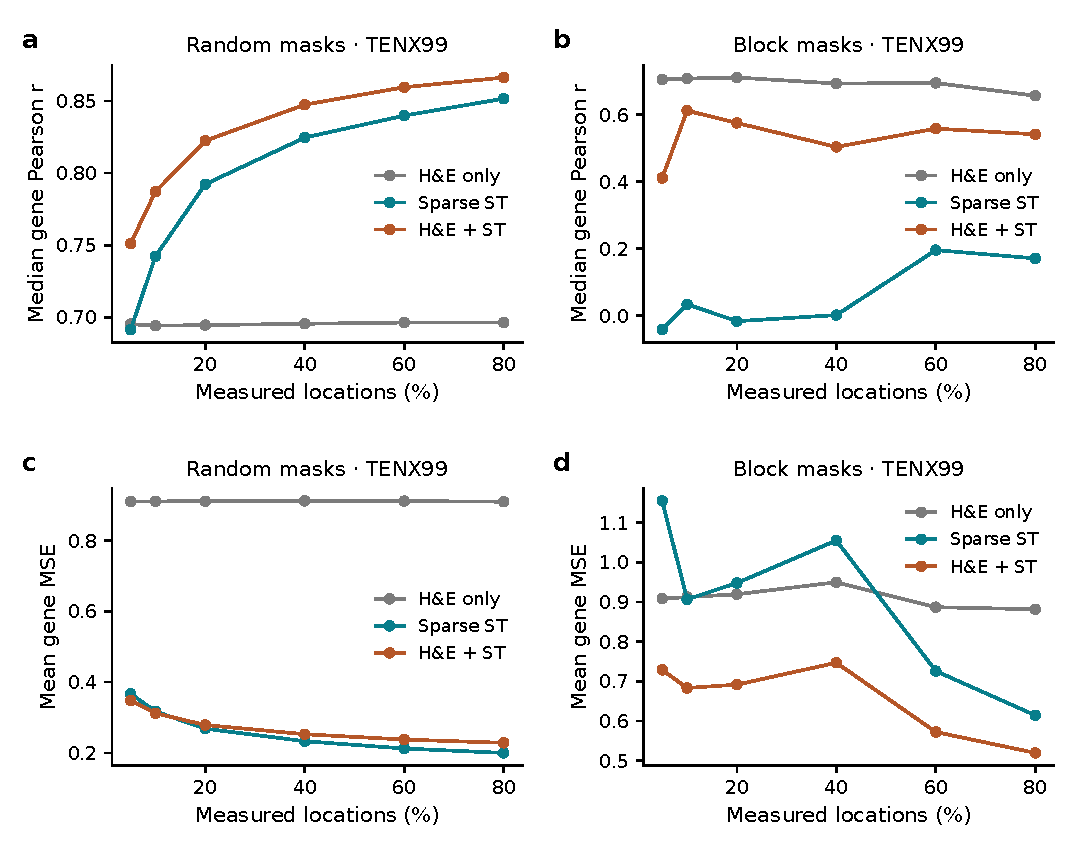
\includegraphics[width=\textwidth,height=0.60\textheight,keepaspectratio]{figures/Figure3.pdf}
\caption{\textbf{Development reconstruction depends on molecular coverage and masking regime.} Results are from the single primary development patient, TENX99, using the frozen 50-gene panel and ResNet18 representation. \textbf{a,c,} Distributed random observation. \textbf{b,d,} The earlier development block-mask regime. Panels a and b show median gene Pearson correlation; panels c and d show mean gene MSE across measurement fractions. The image-only, selected molecular interpolation and fixed fusion curves summarize three frozen mask replicates per condition; curves are means over masks, not patient confidence intervals. Targets and error units are unchanged across methods. The development block masks differ from the external V2 forbidden-region protocol and should not be treated as directly equivalent geometry tests. At 20\% distributed coverage, fusion has higher correlation than interpolation but slightly higher MSE, illustrating that spatial association and calibration are distinct properties. The image-only comparator receives no observed molecular anchors.}
\label{fig:development}
\end{figure}
